%!TEX TS-program = xelatex
\documentclass[notes,12pt, aspectratio=169]{beamer}

\usepackage{amsmath,amsfonts,amssymb,amsthm,mathtools}  % пакеты для математики
%\usepackage{minted}
\usepackage[english, russian]{babel} % выбор языка для документа
\usepackage[utf8]{inputenc} % задание utf8 кодировки исходного tex файла
\usepackage[X2,T2A]{fontenc}        % кодировка

\usepackage{fontspec}         % пакет для подгрузки шрифтов


% why do we need \newfontfamily:
% http://tex.stackexchange.com/questions/91507/
% why do we need \newfontfamily:
% http://tex.stackexchange.com/questions/91507/
\newfontfamily{\cyrillicfonttt}{Georgia}
\newfontfamily{\cyrillicfont}{Georgia}
\newfontfamily{\cyrillicfontsf}{Georgia}


\usepackage{unicode-math}     % пакет для установки математического шрифта
% \setmathfont{Neo Euler} % шрифт для математики

\usepackage{polyglossia}      % Пакет, который позволяет подгружать русские буквы
\setdefaultlanguage{russian}  % Основной язык документа
\setotherlanguage{english}    % Второстепенный язык документа

% Шрифт для кода

\usepackage{verbments}

\usepackage{pgfpages}
% These slides also contain speaker notes. You can print just the slides,
% just the notes, or both, depending on the setting below. Comment out the want
% you want.
%\setbeameroption{hide notes} % Only slide
%\setbeameroption{show only notes} % Only notes
%\setbeameroption{show notes on second screen=right} % Both

\usepackage{array}

\usepackage{tikz}
\usepackage{verbatim}
\setbeamertemplate{note page}{\pagecolor{yellow!5}\insertnote}
\usetikzlibrary{positioning}
\usetikzlibrary{snakes}
\usetikzlibrary{calc}
\usetikzlibrary{arrows}
\usetikzlibrary{decorations.markings}
\usetikzlibrary{shapes.misc}
\usetikzlibrary{matrix,shapes,arrows,fit,tikzmark}

\usepackage{hyperref}
\usepackage{lipsum}
\usepackage{multimedia}
\usepackage{multirow}
\usepackage{dcolumn}
\usepackage{bbm}
\newcolumntype{d}[0]{D{.}{.}{5}}

\usepackage{changepage}
\usepackage{appendixnumberbeamer}
\newcommand{\beginbackup}{
   \newcounter{framenumbervorappendix}
   \setcounter{framenumbervorappendix}{\value{framenumber}}
   \setbeamertemplate{footline}
   {
     \leavevmode%
     \hline
     box{%
       \begin{beamercolorbox}[wd=\paperwidth,ht=2.25ex,dp=1ex,right]{footlinecolor}%
%         \insertframenumber  \hspace*{2ex} 
       \end{beamercolorbox}}%
     \vskip0pt%
   }
 }
\newcommand{\backupend}{
   \addtocounter{framenumbervorappendix}{-\value{framenumber}}
   \addtocounter{framenumber}{\value{framenumbervorappendix}} 
}

% для имитации питоновского синтаксиса 
\newcommand{\pgr}[1]{{\color{green} \textbf{#1}}}


%%%%%%%%%% Работа с картинками %%%%%%%%%
\usepackage{graphicx}                  % Для вставки рисунков
\usepackage{graphics}
\graphicspath{{images/}}    % можно указать папки с картинками
\usepackage{wrapfig}                   % Обтекание рисунков и таблиц текстом

\usepackage[space]{grffile}
\usepackage{booktabs}

% These are my colors -- there are many like them, but these ones are mine.
\definecolor{blue}{RGB}{0,114,178}
\definecolor{red}{RGB}{213,94,0}
\definecolor{yellow}{RGB}{240,228,66}
\definecolor{green}{RGB}{0,128, 0}

\hypersetup{
  colorlinks=false,
  linkbordercolor = {white},
  linkcolor = {blue}
}


%% I use a beige off white for my background
\definecolor{MyBackground}{RGB}{255,253,218}

%% Uncomment this if you want to change the background color to something else
%\setbeamercolor{background canvas}{bg=MyBackground}

%% Change the bg color to adjust your transition slide background color!
\newenvironment{transitionframe}{
  \setbeamercolor{background canvas}{bg=yellow}
  \begin{frame}}{
    \end{frame}
}

\setbeamercolor{frametitle}{fg=blue}
\setbeamercolor{title}{fg=black}
\setbeamertemplate{footline}[frame number]
\setbeamertemplate{navigation symbols}{} 
\setbeamertemplate{itemize items}{-}
\setbeamercolor{itemize item}{fg=blue}
\setbeamercolor{itemize subitem}{fg=blue}
\setbeamercolor{enumerate item}{fg=blue}
\setbeamercolor{enumerate subitem}{fg=blue}
\setbeamercolor{button}{bg=MyBackground,fg=blue,}


% If you like road maps, rather than having clutter at the top, have a roadmap show up at the end of each section 
% (and after your introduction)
% Uncomment this is if you want the roadmap!
% \AtBeginSection[]
% {
%    \begin{frame}
%        \frametitle{Roadmap of Talk}
%        \tableofcontents[currentsection]
%    \end{frame}
% }
\setbeamercolor{section in toc}{fg=blue}
\setbeamercolor{subsection in toc}{fg=red}
\setbeamersize{text margin left=1em,text margin right=1em} 

% списки, которые растягиваются на всю величину слайда 
\newenvironment{wideitemize}{\itemize\addtolength{\itemsep}{10pt}}{\enditemize}


\title[]{\textcolor{blue}{Практический анализ данных и машинное обучение: искусственные нейронные сети}}
\author{Ульянкин Филипп и Соловей Влад}
\date{\today}



\begin{document}

%%% TIKZ STUFF
\tikzset{   
        every picture/.style={remember picture,baseline},
        every node/.style={anchor=base,align=center,outer sep=1.5pt},
        every path/.style={thick},
        }
\newcommand\marktopleft[1]{%
    \tikz[overlay,remember picture] 
        \node (marker-#1-a) at (-.3em,.3em) {};%
}
\newcommand\markbottomright[2]{%
    \tikz[overlay,remember picture] 
        \node (marker-#1-b) at (0em,0em) {};%
}
\tikzstyle{every picture}+=[remember picture] 
\tikzstyle{mybox} =[draw=black, very thick, rectangle, inner sep=10pt, inner ysep=20pt]
\tikzstyle{fancytitle} =[draw=black,fill=red, text=white]
%%%% END TIKZ STUFF

\begin{frame}
\maketitle
\centering \textbf{\color{blue} Посиделка 8:}  Object detection
\end{frame}

\begin{frame}{Agenda} 
\begin{wideitemize}
	\item Быстрая история
	\item YOLO
\end{wideitemize}
\end{frame}



 \begin{transitionframe}
	\begin{center}
		\Huge  История и метрики
	\end{center}
\end{transitionframe}

\begin{frame}{История}
	Вначале подход был следующим - мы вручную придумываем фичи из картинки, потом каким-либо алгоритмом придумываем как выделить на картинке объект. 
	
	Например мы хотим научиться выделять велосипед - нам нужно сначала научиться выделять части велосипеда, потом скользящим окном выделяем область, где больше всего частей было выделено.
	
	Такой подход хорош, но он медленный - мы много раз используем один и тот же алгоритм на одной картинке, а это больно.
	
	Приход нейронных сетей дал возможность использовать "нейронные знания" об изображении.
\end{frame}



\begin{frame}{Метрики}
Качество детекции определяется следующими метриками :
\begin{enumerate}
	\item Bounding box precision - Правильно ли мы подобрали рамочку, не слишком ли она большая/маленькая;
	\item Recall - Все ли мы объекты нашли?
	\item Class precision -  Мы нашли то, что надо или нет?
\end{enumerate}

Еще мы это хотим применять в real time, а для этого нам нужна скорость. Долго скорость была большой проблемой для алгоритмов - для реального времени нам надо более 5ти детекций в секунду.
\end{frame}

\begin{frame}{Метрики}

Но и precision и recall зависят от нашего treshhold, и в точке его считать не очень хорошо. Выход? - посчитаем для каждого уровня отсечения и возьмем площадь под кривой.
\begin{center}
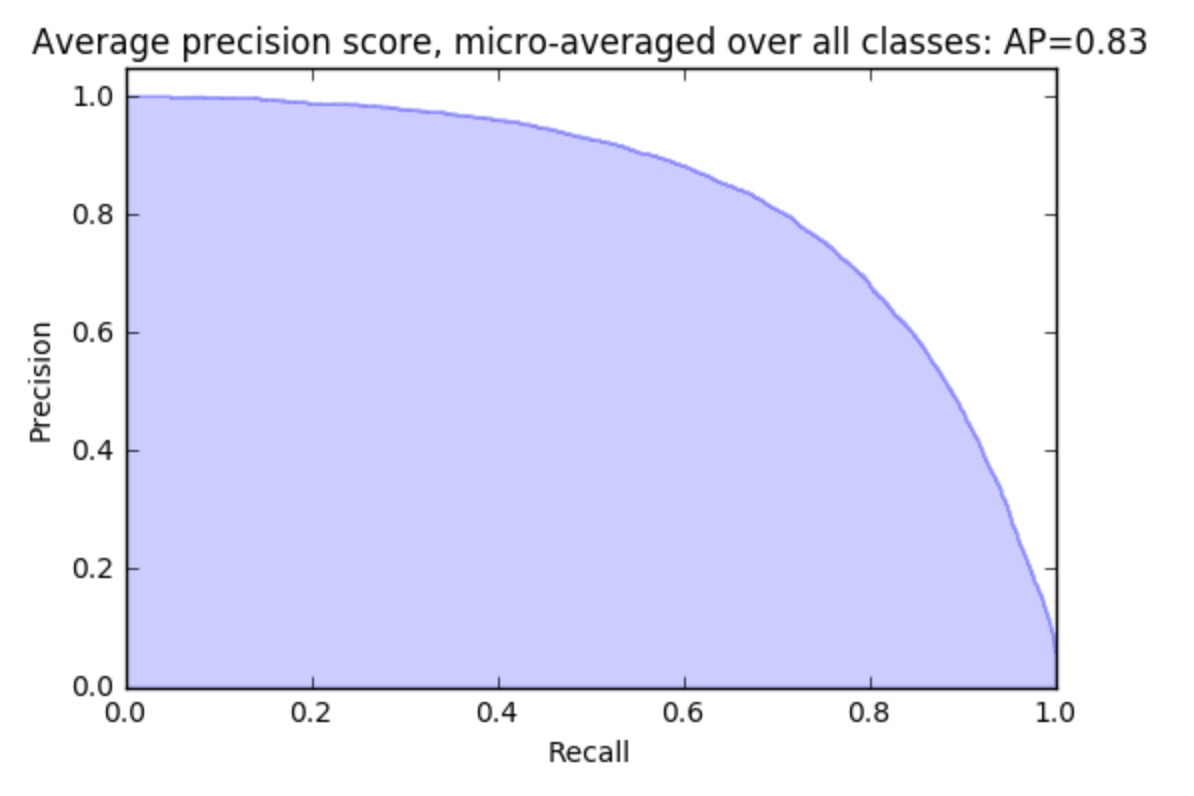
\includegraphics[width=.65\linewidth]{precision_recall.jpg}
\end{center}

\end{frame}

\begin{frame}{Метрики}
	
Осталось научиться считать правильность наших рамочек. Для этого используется следующая метрика - Jaccard index (IoU).

\begin{equation}
	IoU = \cfrac{|A \cap B|}{|A \cup B|} = \cfrac{|A \cap B|}{|A|+|B| - |A \cap B|}
\end{equation}

\begin{center}
	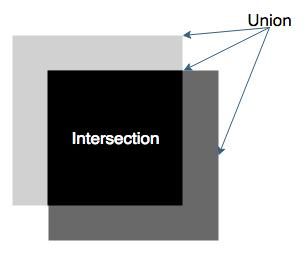
\includegraphics[width=.5\linewidth]{JI.jpg}
\end{center}

\end{frame}


 \begin{transitionframe}
	\begin{center}
		\Huge  YOLO
	\end{center}
\end{transitionframe}


\begin{frame}{YOLO - начало}
	Несколько фактов о YOLO:
	\begin{enumerate}
		\item YOLO-you only look once
		\item Самая быстрая архитектура - 170 рамок в секунду на изображении 256 на 256
		\item Вышла в 2015 году, сейчас уже третья версия из 2018ого
		\item не самая точная, но быстрая за счет небольшой потери качества.
	\end{enumerate}
\end{frame}

\begin{frame}{YOLO - ограничения}
	От чего страдает YOLO - плохо работает с мелкими объектами.
	
	Как пример - Вам будет тяжело выделить отдельную птицу из стаи. 
	
	С этим пытаются бороться, но тяжко. И на краях изображения тоже могут возникнуть проблемы.

\end{frame}

\begin{frame}{YOLO - ключевая идея}
Перевод задачи в простую задачу регрессии. Для каждой рамки мы должны спрогнозировать следующие параметры : 

	\begin{enumerate}
	\item Центр рамки
	\item Ширину и высоту рамки
	\item Вероятность того, что в рамке лежит объект
	\item Ну и класс объекта
\end{enumerate}
Это все чиселки, мы можем считать по ним регрессию! (но пока не будем)
\end{frame}

\begin{frame}{YOLO - ключевая идея 2}
Всю картинку мы покрываем сеткой, из выбираем объекты внутри этой сетки. 

Размер сетки(grid) - наш гиперпараметр. Количество всех возможных рамок - w*h*B(пока оставим за скобками B, тоже наш гиперпараметр)

\begin{center}
	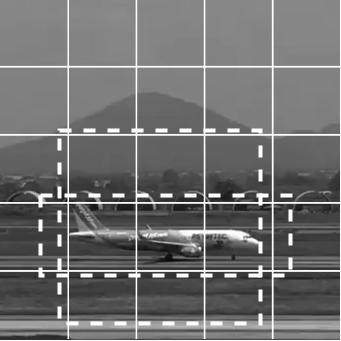
\includegraphics[width=.4\linewidth]{boxes.jpg}
\end{center}
\end{frame}

\begin{frame}{YOLO - вход}
	Начнем разбирать модель с применения.
	
Признаки YOLO обычно берет из других моделей (backbone model). Выбор этой модели влияет на итоговый результат. YOLO берет куб выхода из других моделей.

Итоговая сетка(которая на картинке) зависит от следующих факторов :
	\begin{enumerate}
	\item Насколько сильно снижает размерность модель feature extractor. VGG-16 сжимает в 16 раз (но оставляет 512 каналов)
	\item Входной размер картинки
	
	\begin{center}
	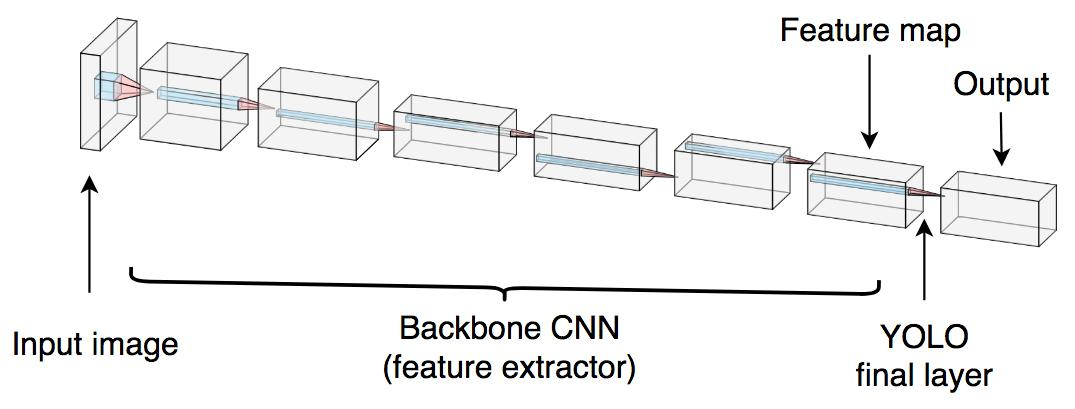
\includegraphics[width=.6\linewidth]{backbone.jpg}
\end{center}
\end{enumerate}

\end{frame}


\begin{frame}{YOLO - выход}
	Итоговый выход YOLO - w*h*M, где M = B*(C+5).
		\begin{enumerate}
		\item С-количество классов, которое у нас всего может быть
		\item B-количество рамок (как их задавать поговорим позже)
	\end{enumerate}
Осталось еще 5 штук:
\begin{enumerate}
	\item $t_x$ и $t_y$ - координаты центра рамки
	\item $t_w$ и $t_h$ - ширина и высота рамки
	\item $c$ - вероятность того, что у нас в рамке вообще что-то есть
	\item ну и $p_1$,.....$,P_C$ - вероятности того, что в рамке лежит объекта класса 1,.... С
\end{enumerate}
	
\end{frame}

\begin{frame}{YOLO - выход}
\begin{center}
	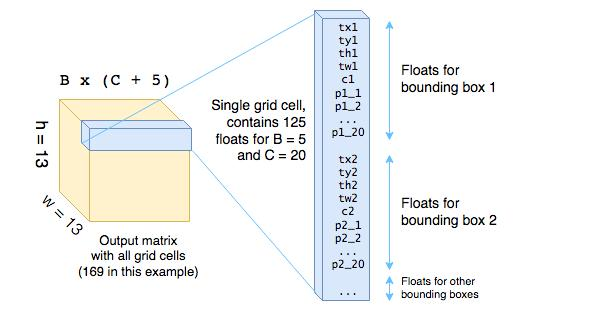
\includegraphics[width=1\linewidth]{output.jpg}
\end{center}
	
\end{frame}


\begin{frame}{YOLO - якорные рамки}
Наконец-то мы поговорим об этом \textbf{B}. Учить ширину, высоту и координаты центра рамки прям в лоб тяжело, объекты слишком разные по размеру. Поэтому мы вводим понятие - якорная рамка и будем немного корректировать эти рамки под конкретные объекты.

На практике таких рамок обычно от 3 до 25. Обычно используют 9 рамок:
\begin{enumerate}
	\item квадратные (Большая, средняя , маленькая)
	\item вертикально-прямоугольные (Большая, средняя , маленькая)
	\item горизонтально-прямоугольные (Большая, средняя , маленькая)
\end{enumerate}
Размеры рамок задаются под наш датасет руками.
	
\end{frame} 




\begin{frame}{YOLO -корректировка рамок}
Рамки корректируются под конкретный объект по следующему правилу:
\begin{enumerate}
	\item $b_x = sigmoid(t_x)+c_x$
	\item $b_y = sigmoid(t_y)+c_y$
	\item $b_w = p_w * exp(t_w)$
	\item $b_h = p_h * exp(t_h)$
\end{enumerate}
 Где:
 \begin{enumerate}
 	\item $t_x$,$t_y$,$t_w$,$t_h$ - выход последнего слоя
 	\item $b_x$,$b_y$,$b_w$,$b_h$ - итоговая оценка рамок
 	\item $p_w$,$p_h$ - размеры якорной рамки
 	\item $c_x$,$c_y$ - координаты конкретного места в сетке, где мы нашли рамку (включаются на границе)
 \end{enumerate}
\end{frame}

\begin{frame}{YOLO -корректировка рамок}
\begin{center}
 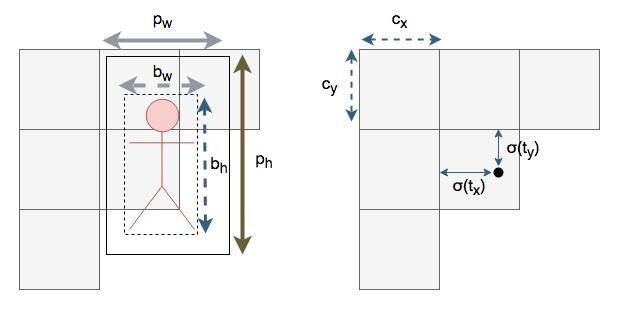
\includegraphics[width=1\linewidth]{corrections.jpg}
\end{center}
\end{frame}



\begin{frame}{YOLO -пост-процессинг рамок}
У нас получилось огромное количество рамок - надо их как-то отобрать.

Для начала выкидываем все, вероятность нахождение объекта в которых ниже определенной грани (опять же сами выбираем уровень).

Потом оставляем рамки с объектом, который принадлежит классу с наибольшей вероятностью. Получается следующая картинка:
\begin{center}
 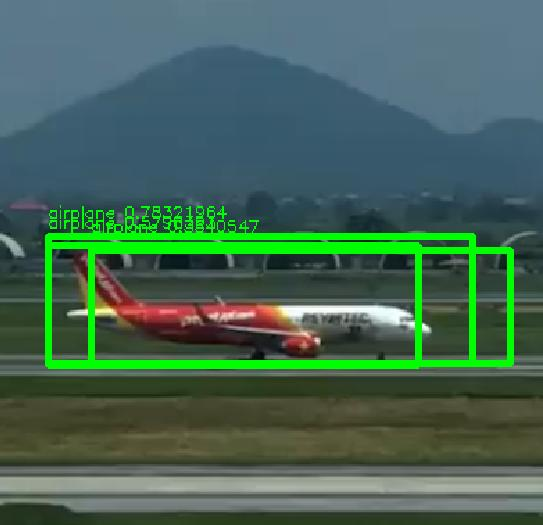
\includegraphics[width=.4\linewidth]{full_boxes.jpg}
\end{center}
\end{frame}

\begin{frame}{YOLO -NMS}
NMS - Non-max suppression.

Выкидываем все рамки, у которых $IoU$ ниже какого-то порога (мы сами его выбираем). И следующим шагом выбираем рамку, у которой $IoU$ имеет максимальное значение.

\begin{center}
 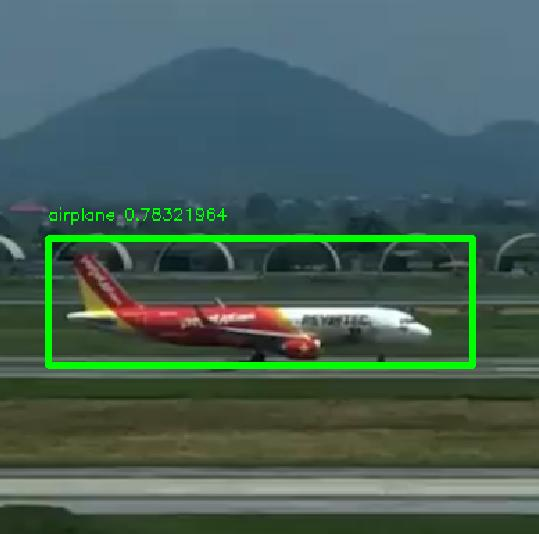
\includegraphics[width=.4\linewidth]{NMS.jpg}
\end{center}
\end{frame}



\begin{frame}{YOLO - Подводим итоги применения}

 \begin{enumerate}
	\item Считаем карту признаков через backbone CNN
	\item Считаем через сверточный слой корректировку для якорных рамок, вероятности нахождения объекта в рамке и вероятность класса внутри рамки.
	\item Корректируем размеры нашей рамки
	\item Отбираем наши рамки.
\end{enumerate}


\end{frame}

\begin{frame}{YOLO - Подводим итоги применения}


\begin{center}
 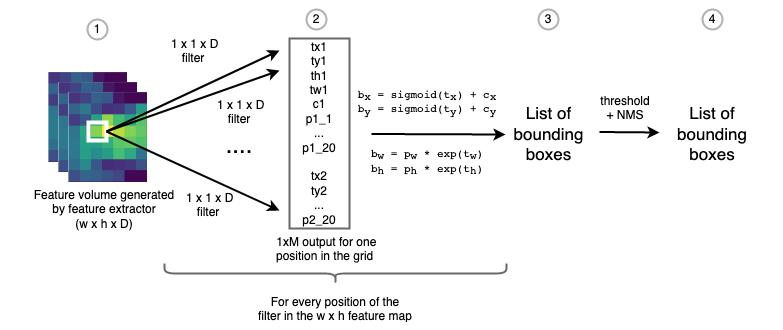
\includegraphics[width=1\linewidth]{final_interfece.jpg}
\end{center}

\end{frame}


\begin{frame}{YOLO - обучение}

Модель backbone  к нам приходит откуда угодно. Обычно учат на большом дата сете (типа imagenet) и потом используют. 

Можно учить все сразу, но это больно (вот прям совсем больно). Можно предобучать как автоэнкодер.

Специально для YOLO была разработана архитектура, которая наиболее эффективно выделяет фичи из картинки (по словам авторов статей). Данная структура называется Darknet. И да - основная модельная сложность в экстракторе фичей, если хотим использовать на мобилке, уменьшаем сложность этой модели.

\end{frame}

\begin{frame}{Bounding box loss}
\begin{center}
 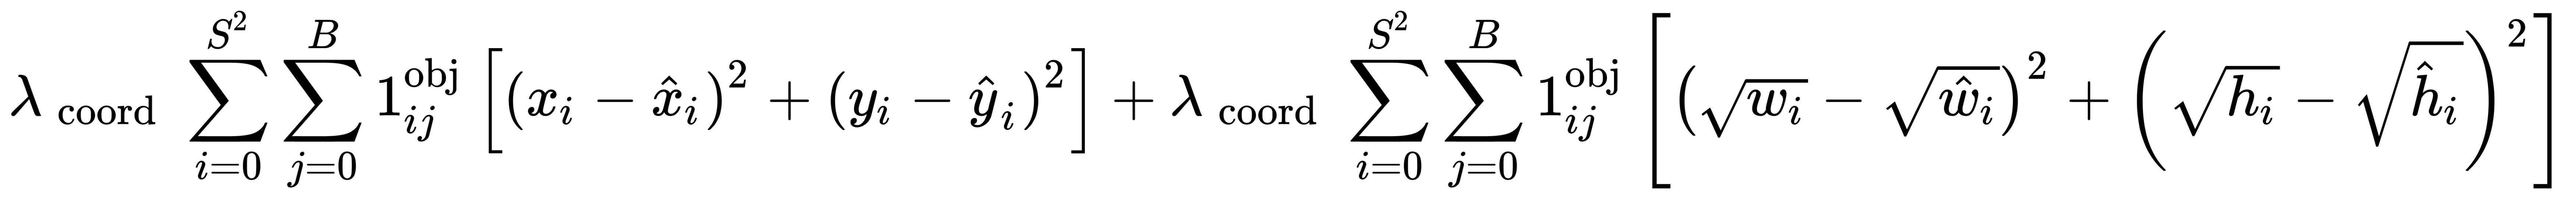
\includegraphics[width=1\linewidth]{bounding_box_loss.jpg}
\end{center}

Где
 \begin{enumerate}
	\item $\lambda$ - насколько сильно мы хотим сконцентрироваться на рамках в итоговых потерях
	\item $1^{obj}_{ij}$ - индикаторная функция, которая 1 если найденная рамка отвечает за объект. Из всех рамок выбирается рамка с наибольшим $IoU$.
	\item Корень нам дает штраф на маленьких рамках больше, чем на больших
\end{enumerate}
\end{frame}

\begin{frame}{Object confidence loss}
\begin{center}
 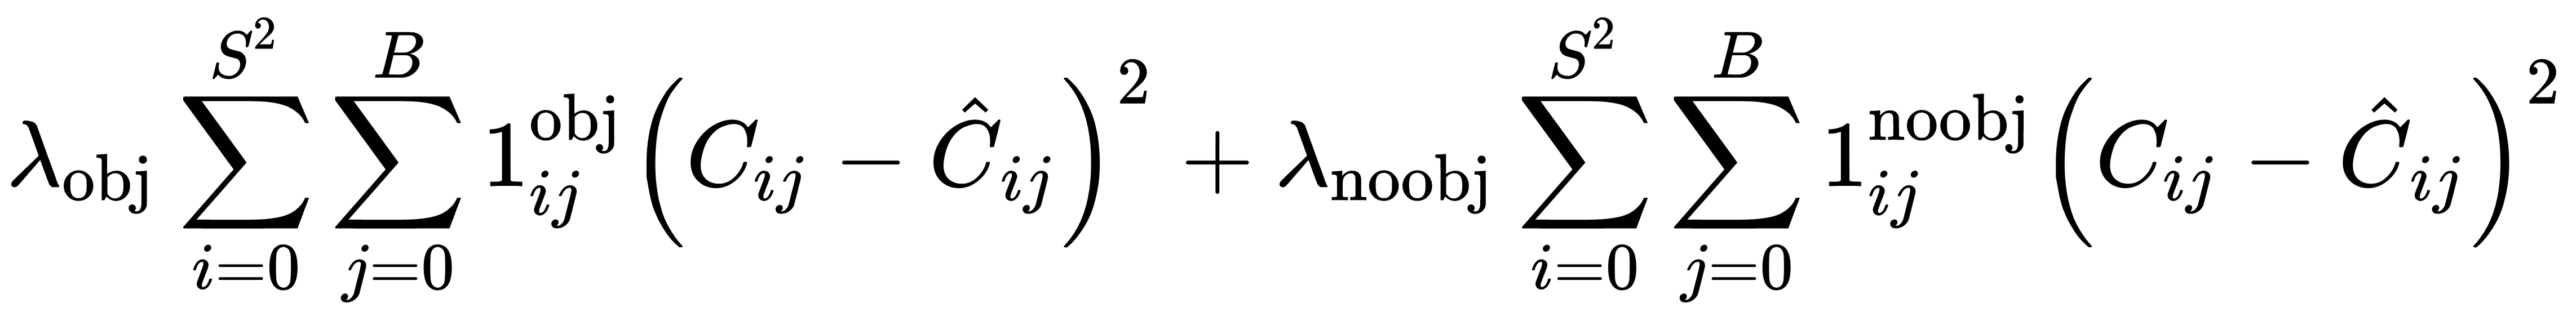
\includegraphics[width=0.8\linewidth]{object_loss.png}
\end{center}

Где
 \begin{enumerate}
	\item $\lambda$ - все также вес в итоговых потерях
	\item $C$ - содержит ли рамка вообще объект 
	\item $1^{noobj}_{ij}$ - индикаторная функция, которая 1 если найденная рамка никак не относится к объекту.
	
\end{enumerate}
\end{frame}

\begin{frame}{Classification loss}
\begin{center}
 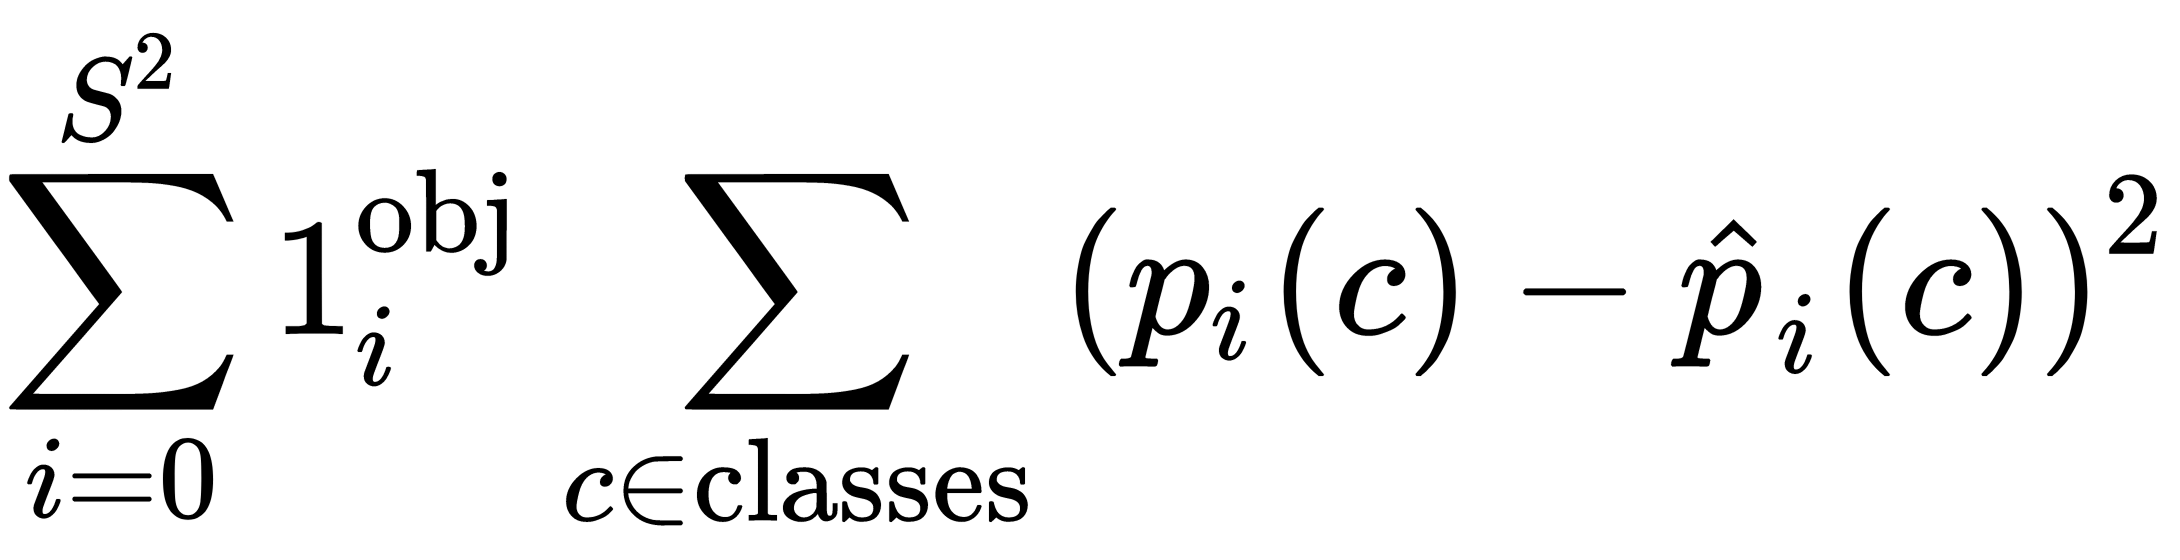
\includegraphics[width=0.6\linewidth]{class_loss.png}
\end{center}

Тут все просто - угадали или нет с объектом.
	
Итоговый наш лосс - это сумма всех трех потерь сразу.

\end{frame}

\begin{frame}{Несколько хинтов при обучении}
\begin{center}
 \begin{enumerate}
	\item Аугументация данных и dropout - обязательные куски, без них сетка сразу переобучается.
	\item Каждый n эпох меняем входную размерность изображения, чтобы научить сеточку быть независимой от размерности
	\item Предобучаем сеточку, все вместе не учим - ну очень больно
	\item Градиент может взорваться - следим за этим. 
	
\end{enumerate}
\end{center}

\end{frame}

\begin{frame}{Итого}
Всей этой историей хотелось показать следующее - есть отдельные кусочки из которых состоят нейронки (свертки, dropout, batchnorm...), а есть отдельные архитектуры в которых очень много неочевидных хаков.

И прям учить архитектуры - плохая идея, слишком они быстро меняются и зависят от данных.

\end{frame}

\end{document}
